\documentclass[11pt,twoside,a4paper]{article}
\usepackage[margin=20pt]{geometry}
\usepackage{tabu}
\usepackage{amsmath}
\usepackage{enumitem}
\usepackage{graphicx}
\newcommand{\norm}[1]{\left\lVert#1\right\rVert}
\newcommand\ceil[1]{\lceil#1\rceil}

\begin{document}
\title{Using GPU as an accelerator}
\author{Anil Shanbhag}
\maketitle

There is a lot of excitement around using accelerators like GPU and FPGAs to
accelerate analytics. In fact, in the recent VLDB, two of the keynotes I
attended  (one by Ion and other by Gustavo) were centered around this theme. 

GPUs have been widely adopted to do deep learning. However, GPUs also have a lot of
potential to accelerate memory-bound applications like the ones we considered in
NVL. There are two main contributing factors for why GPU's are appealing now:

1) The latest generation of GPU's have large amount of memory (the latest K80
Tesla card has 24GB memory, 3 years ago most papers had graphics card with at
max 4 GB memory) and significantly higher memory bandwidth than a CPU (CPU
bandwidth ~ 60 GBps compared to 480 GBps in K80). On a local machine with Titan
X GPU, we observed a memory bandwidth of 280 GBps on GPU (listed as max 330 GBps
in device spec) compared to 47GBps on CPU. The PCIe transfer speed is much
slower. As a result, all the works so far, which had to ship data from CPU to
GPU, suffered from limited gains as PCIe transfer time becomes the bottleneck.
The large memory allows us to keep/cache all or a good fraction of the dataset
on the GPU itself, eliminating the PCIe transfer overhead. 

2) GPUs are becoming commodities. Azure recently launched the N-series which are
machines with GPUs. The largest of them comes with 2 K80 cards having an
aggregate of 48GB GPU memory. The price point is $\$2.48ph$ for 24 cores/224GB
RAM in addition to 2 GPUs. This is comparable to $\$1.83$ for 20 core/140GB RAM
machine with no GPU. More cards can be stacked, MapD has machines with 8 K80
cards attached on the same machine. 

There are a number of exciting research directions. 

\section{Generating Optimized Code}

\begin{figure}[!h]
  \centering
    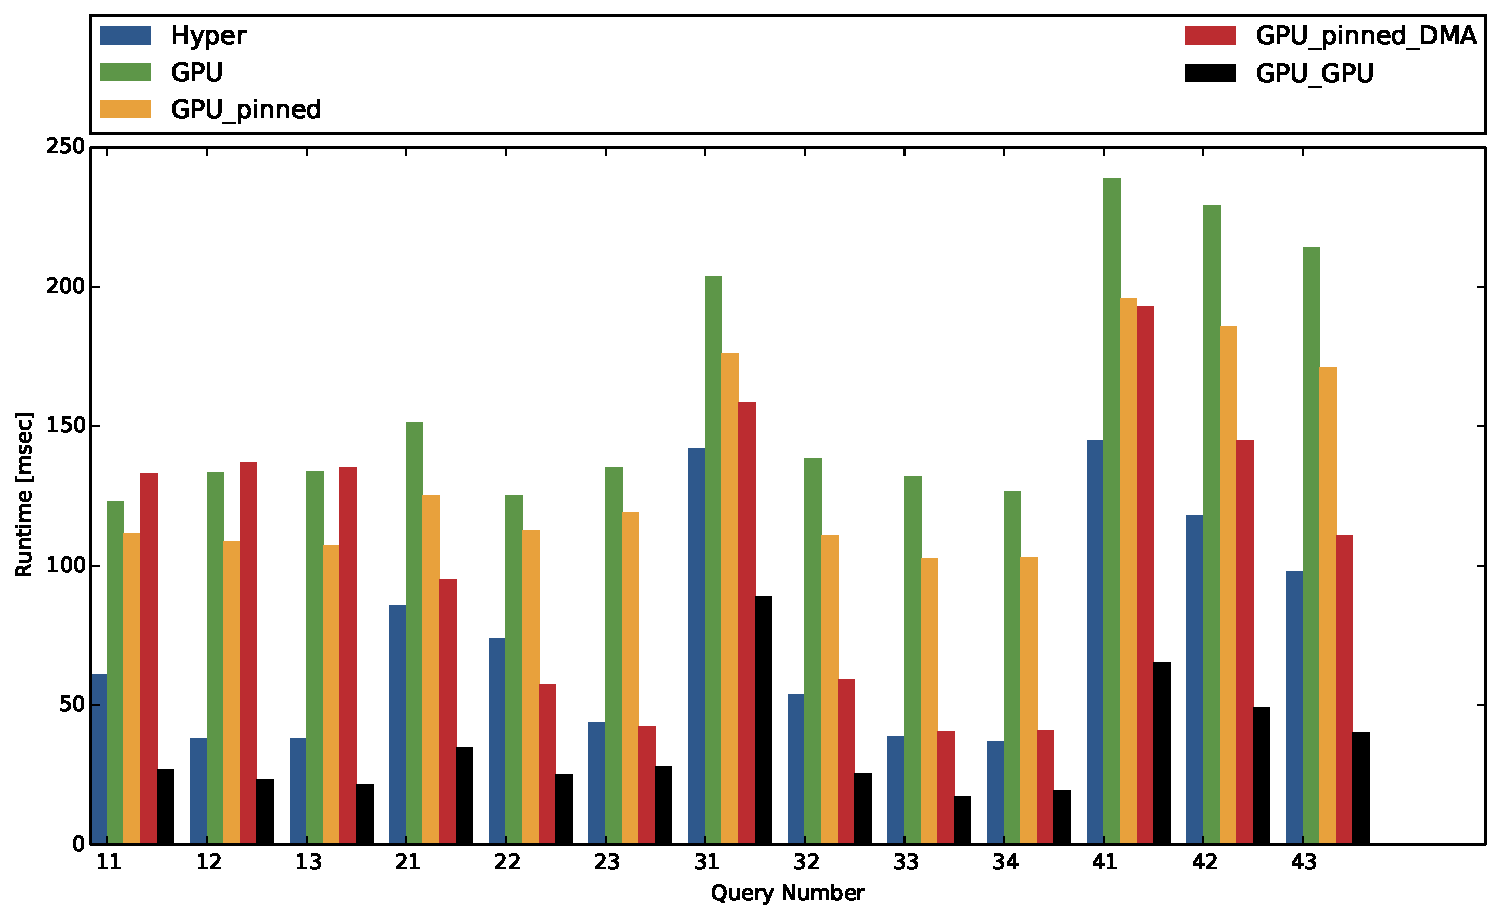
\includegraphics[width=0.9\textwidth]{runtimes.pdf}
  \caption{Comparing performance.}
  \label{fig:runtimes}
\end{figure}

GPUs can theoretically accelerate analytics applications. In figure
\ref{fig:runtimes}, we took the GPUDB database which was used in
\cite{gpudb,gpudb2} on the star schema benchmark and compared its performance
against Hyper. The paper compared the performance against MonetDB back in 2013
and observed atleast 2x performance improvement with data stored in main memory.
Much has changed since then, with improved algorithms for joins and query
compilation pioneered by Hyper, main-memory databases are almost always
memory-bound. The figure contains 4 modes in which GPUDB ran:
\begin{itemize}
\item GPU: data is on host and in paged memory
\item GPU pinned: data is on host and in pinned memory
\item GPU pinned DMA: data is on host, in pinned memory and data transfer done
via DMA
\item GPU GPU: data is on GPU 
\end{itemize}
We observed that GPUDB never performs better than Hyper when data is in main
memory and the gain is nowhere close to the bandwidth ratio when data is on GPU.
In a hand-tuned implementation we observed greater than 5x gain for q11,q12,q13.
There is a need to generate better code targetted for GPU. As machine learning
applications already default to using GPUs, there is scope to do all-in GPU with
cross library optimization.

\section{Algorithms}

There has been considerable research on optimizing standard relational operators
for main-memory databases. The same is not true for GPUs. There is still
considerable room on coming up with better algorithms and deciding what is the
algorithm to use for each operation. One operator I looked at so far is Top-k. 
On CPU, a sequential version can be done using a priority queue to have
$O(n logk)$. On the GPU, everyone just does a sort followed by selecting the top k
entries. I have a sketch of an algorithm that has a $O(n (log k)^2)$ work
complexity and $log k$ delay. There is probably some tricks to implement it
efficiently and do come with similar algorithms for other operations.

\section{Heterogenous Computing}

Going back to the Azure VM, the machine has 20 cores, 224GB RAM and 2 K80 with
48GB RAM in total. Complete utilization of the machine requires using both CPU
and GPU resources. There are a number of ways to do this. There are a number of
ways to look at the problem too.

Scope
\begin{itemize}
\item Look at relational operations
\item Look at general operators a.la tensorflow
\end{itemize}

Where is the data
\begin{itemize}
\item Data is split between GPU and CPU
\item There are two copies of data: one on CPU, one on GPU
\item Data is only on the CPU, moved to GPU
\end{itemize}

How to partition
\begin{itemize}
\item Horizontally partition the problem, process fraction of the data on GPU /
fraction on CPU
\item Look at inter-operator parallelism
\item Look at query level parallelism: Query gets scheduled on GPU or CPU
\end{itemize}

The specific case I am looking at is relational operators with data being on the
CPU. We will attempt to run the incoming query on the GPU and move/cache the
columns used on the GPU. They are not deleted. When a subsequent query wants to
run on the GPU, it will move any additional columns to the GPU in order to
execute. Since many queries might access the same columns, we save on the
transfer cost by caching it. When we exhaust the GPU memory, we can replace an
existing column with the needed column. This is similar to caches in CPU land,
but the difference is that there is one full copy of the data on the CPU. So, if
the query requires many new columns which we predict maybe by forcasting will
not be used in future, we can execute the query on CPU and avoid moving out
columns from the GPU.

There is no good open-source GPU-based database. The database resulting from
this effort could be an useful resource. NVL could be a good substrate for
compiling the query plans.



\section{Cost Modelling}

It turns out Tensorflow does not have any cost model. Atleast there is no such
thing in the public release. User has to manually place computation on different
devices. There has been some work on cost modelling of relational operators for
GPU operators \cite{gpudb}. This was relatively easy due to the small number of
operators. For arbitrary operators, it can possibly be done but would require
much more work.

\subsection{Selection}

Symbols:

\begin{itemize}[label={},noitemsep]
\item $B_r$ - read bandwidth of global memory
\item $B_w$ - write bandwidth of global memory
\item $C_r$ - read segment size of global memory
\item $C_w$ - write segment size of global memory
\item $W$ - number of threads in the thread group
\item $\norm{R}$ - cardinality of table R
\item $n$ - number of projected columns
\item $K_i$ - attribute size of the ith projected column
\item $m$ - number of predicate columns
\item $P_i$ - the attribute size of the ith predicate columns
\item $r$ - selectivity of the predicates
\end{itemize}

\noindent \textbf{Old Model}: Scan and write out filter per column with predicate
\begin{align*}
T_1 &= \sum_{i=1}^{m} ( \ceil{\frac{P_i W}{C_r}} + \ceil{\frac{4 W}{C_r}} ) \times \frac{\norm{R}}{W} \times \frac{C_r}{B_r}  +  \sum_{i=1}^{m} \ceil{\frac{4 W}{C_w}} \times \frac{R}{W} \times \frac{C_w}{B_w}
\end{align*}
Read the filter and write results to global memory.
\begin{align*}
T_2 &= \sum_{i=1}^{n} (\ceil{\frac{4 W}{C_r}} + \ceil{\frac{K_i}{4}}) \times \frac{\norm{R}}{W} \times \frac{C_r}{B_r} + \norm{R} \times r \times \sum_{i=1}^{n} \ceil{\frac{K_i}{4}} \times \frac{C_w}{B_w}
\end{align*}

\noindent \textbf{New Model}: Scan all the columns and write out the filter
\begin{align*}
T_1 &= \sum_{i=1}^{m} \ceil{\frac{P_i W}{C_r}} \times \frac{\norm{R}}{W} \times \frac{C_r}{B_r}  +  \ceil{\frac{4 W}{C_w}} \times \frac{R}{W} \times \frac{C_w}{B_w}
\end{align*}
Read the filter and write results to global memory.
\begin{align*}
T_2 &= (\ceil{\frac{4 W}{C_r}} + \sum_{i=1}^{n} \ceil{\frac{K_i}{4}}) \times \frac{\norm{R}}{W} \times \frac{C_r}{B_r} + \sum_{i=1}^{n} \ceil{\frac{r R K_i}{C_w}} \times \frac{C_w}{B_w}
\end{align*}

\noindent \textbf{CPU Model}:

%\begin{center}
%\begin{tabu} to \textwidth { |X| X| X| }
 %\hline
 %Old Model & New Model & CPU Model \\ 
 %\hline




 %& cell5 

 %& cell6 \\  
 %\hline
 %cell7 & cell8 & cell9 \\ 
 %\hline
%\end{tabu}
%\end{center}



\bibliographystyle{abbrv}
\bibliography{references}

\end{document}
